% !TEX root = main.tex

\section{2D vortex-in-cell problem}~\label{App_2D}
\subsection{Description of the method}


In this section, we apply the Vortex Method in a two-dimensional scenario, as outlined by Cottet et al. \cite{cottet_vortex_2000}. The Vortex Method is a Lagrangian approach utilizing a particle ensemble to discretize the vorticity field, allowing for the solution of the Navier-Stokes equation for viscous incompressible flow. The method is grounded in the vorticity-velocity formulation of the Euler equation, where $\bm \omega = \nabla \times \bm{v}$ satisfies

\[
	\begin{aligned}
		\frac{\partial \bm \omega}{\partial t} + (\bm{v} \cdot \nabla) \bm \omega - \nu \Delta \bm \omega & = 0, \\
		\nabla \cdot \bm v                                                                                & = 0,
	\end{aligned}
\]Where $\omega$ denotes vorticity, $\bm{v}$ represents velocity, and $\nu$ stands for viscosity.

In the context of 2D flow, vorticity is perpendicular to the flow plane, forming a scalar field denoted as $\omega$. In Cartesian coordinates, it is expressed as $\omega = \frac{\partial v_y}{\partial x} - \frac{\partial v_x}{\partial y}$.

The vorticity field is discretized using a collection of discrete vortices, each characterized by a position $\bm z_p$, an associated kernel $\varphi_p$, and a circulation $\Gamma_p$. For all points $\bm z$ within the domain $\Omega$, the vorticity is expressed as

\begin{equation*}
	\omega(\bm z) = \sum_{i=1}^{N_p} \Gamma_p \varphi_p(\bm z - \bm z_p).
\end{equation*}

To address the Navier-Stokes equation, we employ a viscous splitting scheme, following the methodology outlined in \cite{cottet_1990}, acknowledging the predominance of the convection term over viscosity. The initial phase involves solving the advection component for each particle in a Lagrangian context

\begin{eqnarray*}
	\frac{d\bm z_p}{dt} = \bm{v}(\bm z_p), \quad \frac{\omega_p}{dt} = 0.
\end{eqnarray*}~The particle trajectory depends on the local velocity field obtained using the Biot-Savart law. The resolution is based on the Vortex-In-Cell algorithm \cite{christiansen_1973, birdsall_1969}, coupled with an FFT solver to enhance computation performance.

The subsequent steps involve assigning particle vorticity values to the grid using a particle-to-grid formula, computing the velocity field by solving the Poisson equation on the grid verified by the stream function. Finally, the velocity is interpolated back onto the particles using the grid-to-particles formula.

In conclusion, a Runge-Kutta 3 time-stepping scheme is employed to update the particle positions through a time integration scheme. The second phase involves solving the heat equation.
\begin{equation*}
	\frac{d\z_p}{dt} = 0, \quad	\frac{d\omega_p}{dt} = \nu \Delta \omega(\z_p),
\end{equation*}~by employing an integral equation that approximates $\Delta \omega$

\begin{equation*}
	\Delta \omega \approx \varepsilon^{-2} \int [\omega(\z)  - \omega(\bm{y})] \eta_\varepsilon(\bm{y} - \z) d\z,
\end{equation*}

This leads, with the particle approximation, to a redistribution of the particles' intensities in their previous locations, such as

\begin{equation*}
	\frac{d\Gamma_p}{dt} = \nu \varepsilon^{-2} \sum_q (G_q - G_p) \eta_\varepsilon(\z_q - \z_p)
\end{equation*}
For further details on the computation, please refer to \cite{cottet_1990}. Consequently, our vortex model equation is solely dependent on the fluid's viscosity as a model parameter.


\subsection{Lamb-Chaplygin dipole and simulation parameters}

We define the reference as the advection of the Lamb-Chaplygin dipole inside a close domain with stress-free walls. Lamb-Chaplygin dipole is a popular choice for numerical studies \cite{orlandi_vortex_1990}. The model represents a specific steady, inviscid dipolar vortex flow and offers a non-trivial solution to the two-dimensional Euler equations. The dipole is characterized by a translation velocity $U$, a mean position $\bm{z_0}$, a radius $R$, and an orientation $\theta$. This particular test case is designed to assess the impact of a relatively small domain of the particle support, which is crucial for the Part-EnKF filter.

The dipole vorticity field $\omega$ could be expressed as

\begin{equation*}
	\omega(r) = \begin{cases}
		\frac{-2 k U J_1(kr)}{J_0(kR)} \sin \theta, \quad & \text{for} \quad  r < R, \\
		0, \quad                                          & \text{otherwise},
	\end{cases}
\end{equation*}~where $(r, \theta)$ represent the polar coordinates in the dipole reference frame. Here, $J_0$ and $J_1$ denote the zeroth and first order Bessel functions of the first kind, respectively, and $k$ is determined such that $kR$ corresponds to the first non-trivial zero of the first Bessel function.  The dipole vorticity field is depicted in Figure \ref{fig:lamb_dipole}.

\begin{figure}[ht]
	\centering
	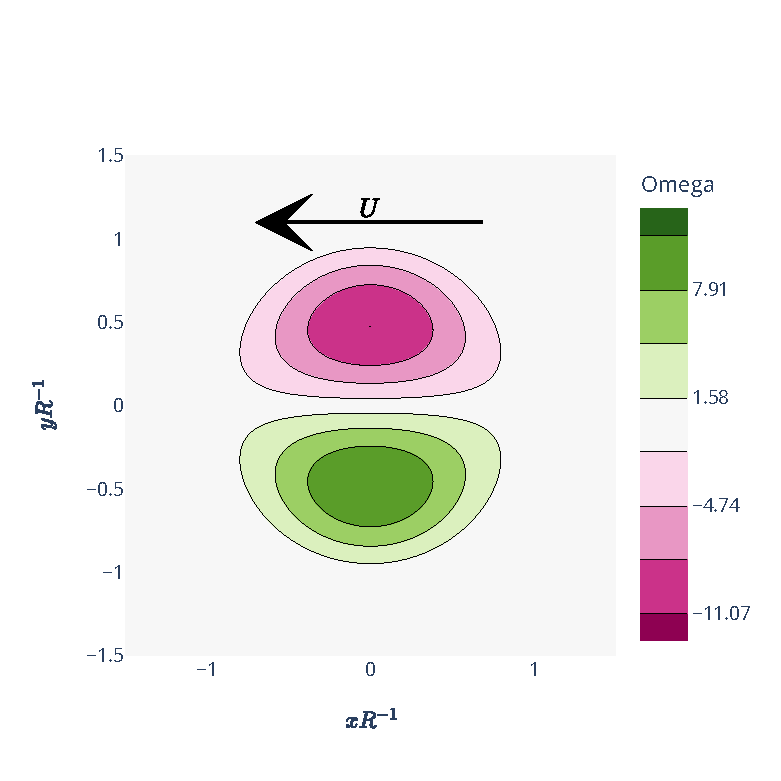
\includegraphics[width=0.6\linewidth]{images/app2d/lamb.pdf}
	\caption{The Lamb-Chaplygin dipole vorticity field on a normalize space.}
	\label{fig:lamb_dipole}
\end{figure}

The dipole is positioned at the center of a box with dimensions $[0, \pi] \times [0, \pi]$, featuring an orientation of $\frac{7\pi}{8}$ rad., a radius of $0.5$ meters, and a velocity $U$ of $0.25 \text{ m.s}^{-1}$. The complete reference setting is listed in Table \ref{tab:ref}.

The boundary box features stress-free walls, meaning fluid cannot pass through them. The velocity perpendicular to the walls is zero, while tangential velocity remains undetermined. When a vortex, such as a dipole, reaches this boundary, it walks along the wall, sensing its reflection and interacting with it.

Because this problem does not have an explicit solution on a closed domain, we simulation the ground truth with a the vortex method for a fined discretization and fixed set of parameters described also in Table \ref{tab:ref}. This is typically referred to as a twin experiment. The trajectory of the ground truth is illustrate in the Figure \ref{fig:ref_trajectory} on a regularly spaced grid.

\begin{figure}[htbp]
	\begin{subfigure}{0.32\textwidth}
		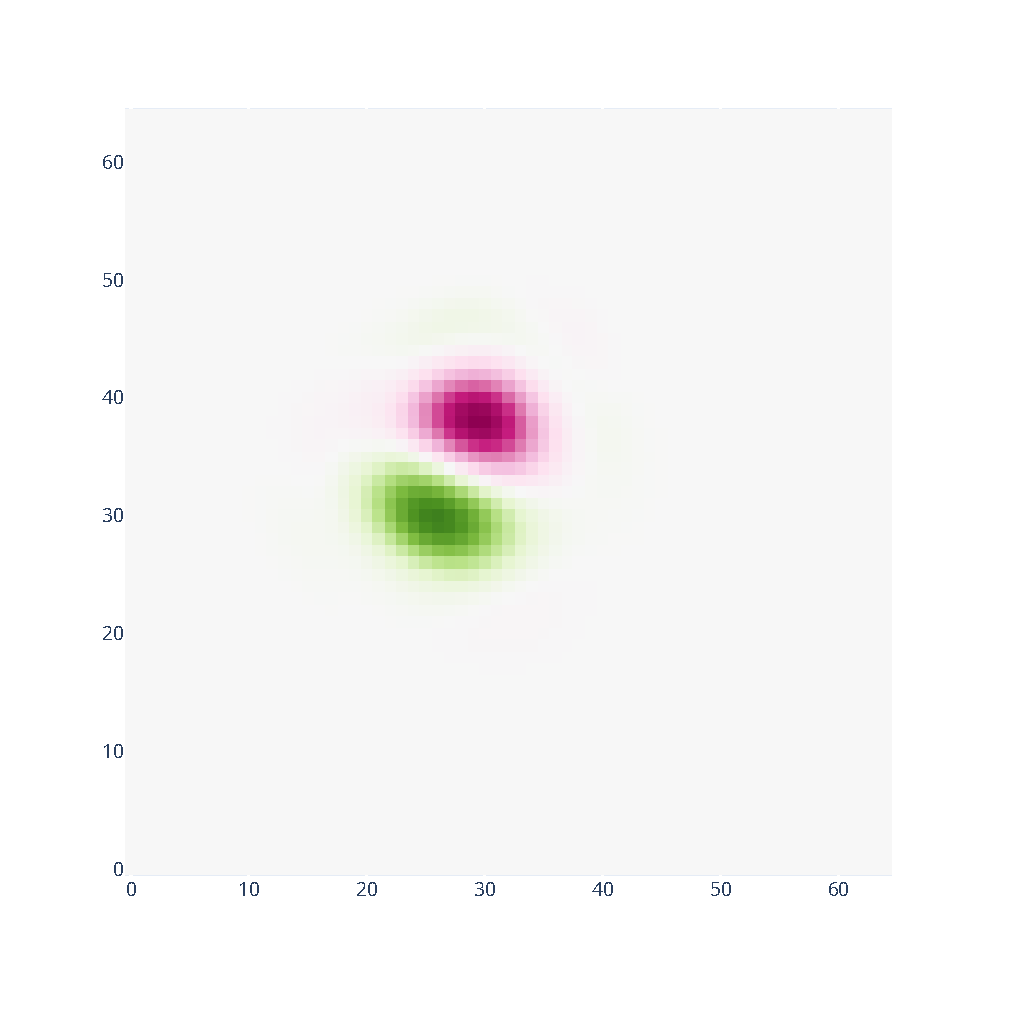
\includegraphics[width=\linewidth]{images/app2d/best_estimate_2.pdf}
	\end{subfigure}
	\hfill
	\begin{subfigure}{0.32\textwidth}
		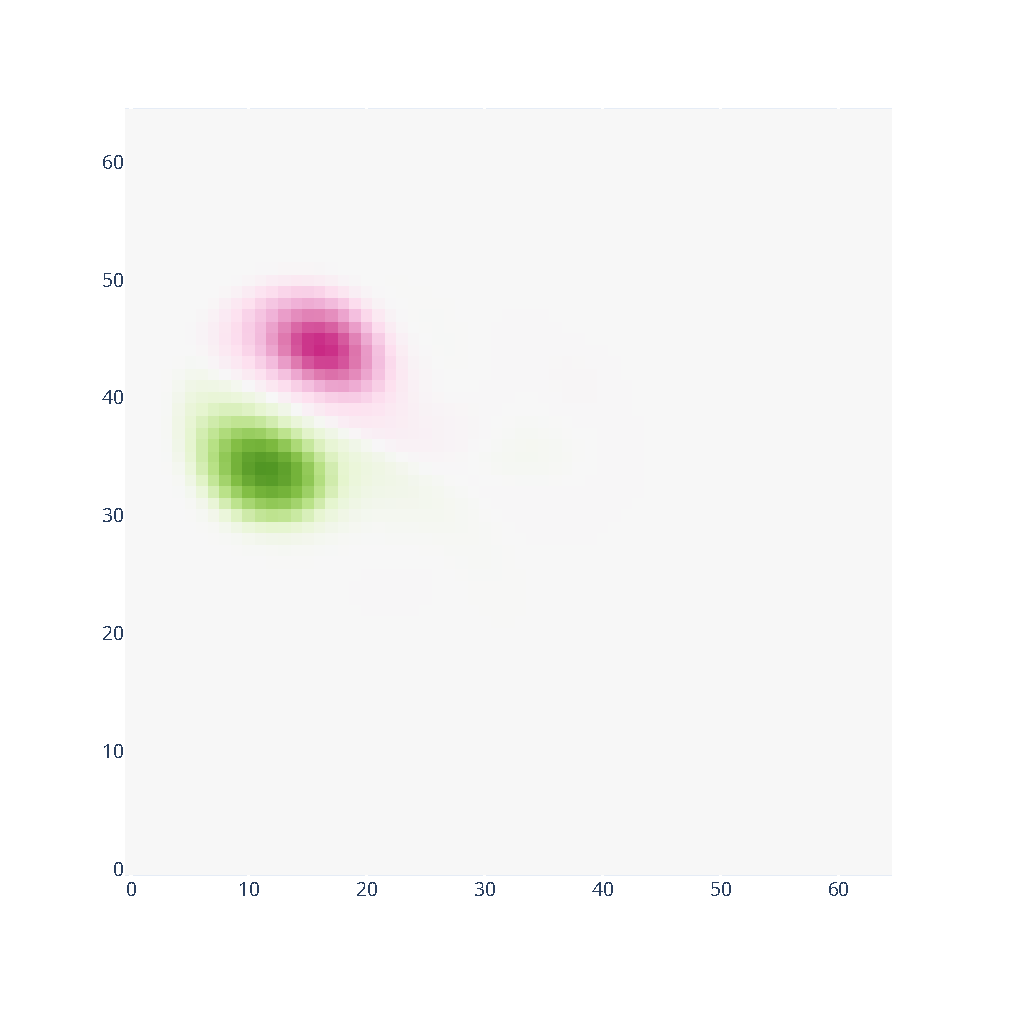
\includegraphics[width=\linewidth]{images/app2d/best_estimate_10.pdf}
	\end{subfigure}
	\hfill
	\begin{subfigure}{0.32\textwidth}
		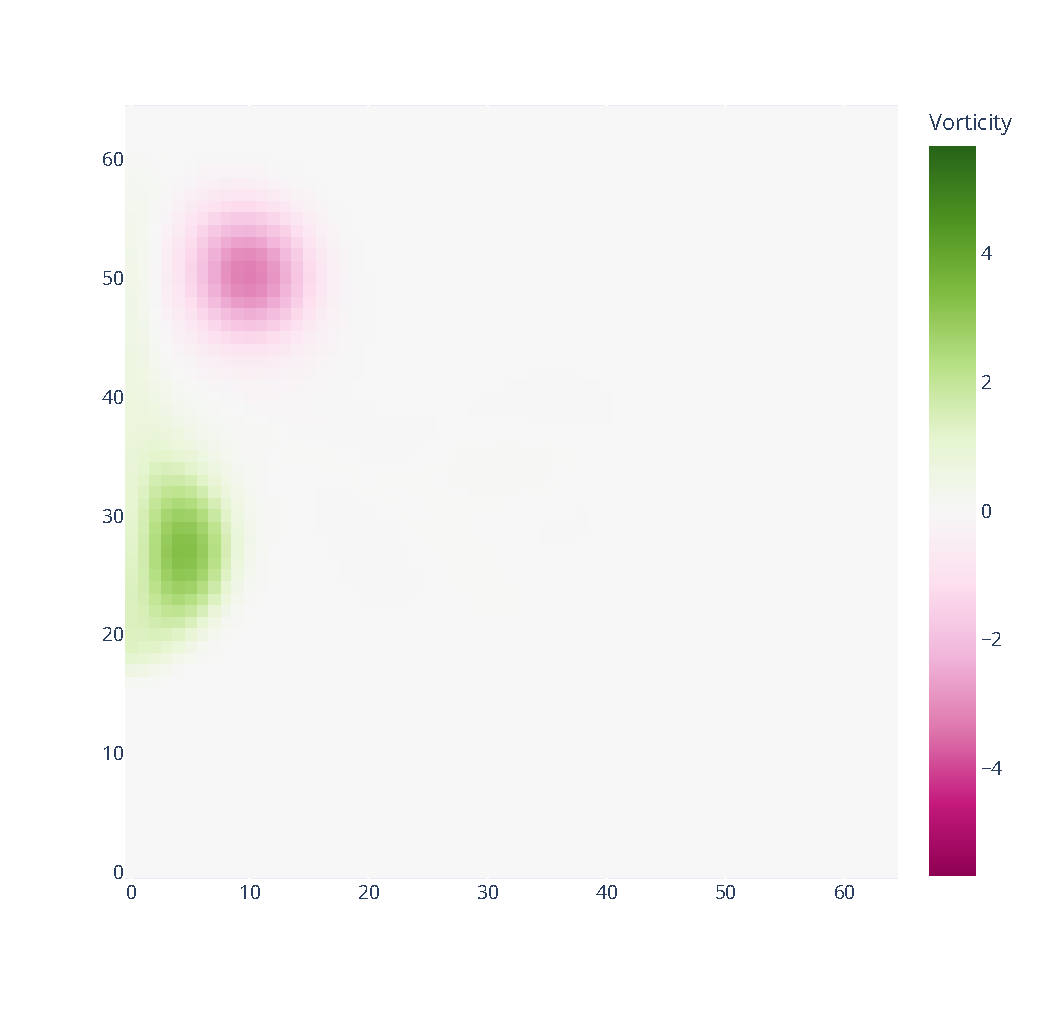
\includegraphics[width=\linewidth]{images/app2d/best_estimate_20.pdf}
	\end{subfigure}
	\caption{Trajectory of the ground truth. The vorticity is represented on a regularly spaced grid. For $t=[1, 5, 10]s.$}
	\label{fig:ref_trajectory}
\end{figure}
Several parameters in the simulation influence the particle distribution and can lead to different results. The first one is the particle size defined by $d_p$, determining the particle volume as $d_p^2$. Another significant parameter is $\varepsilon_\omega$, associated with the remeshing process occurring either during the forecast (to prevent high distortion of the particle distribution) or during the Remesh-EnKF filter. $\varepsilon_\omega$ serves as a threshold, determining whether a particle is retained after the remeshing process based on the condition $V_p \Gamma_p > \varepsilon_\omega$. The impact of this parameter is illustrated for one member after the first forward in Figure~\ref{fig:eps_effect}.

\begin{figure}[htbp]
	\centering
	\begin{subfigure}{0.3\textwidth}
		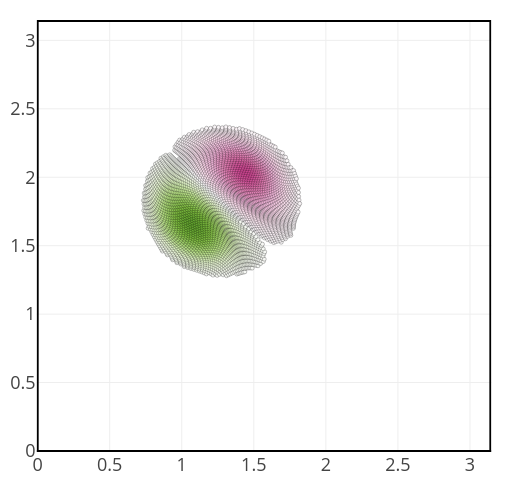
\includegraphics[width=\linewidth]{images/app2d/part_eps_0.1.png}
	\end{subfigure}
	\hfill
	\begin{subfigure}{0.3\textwidth}
		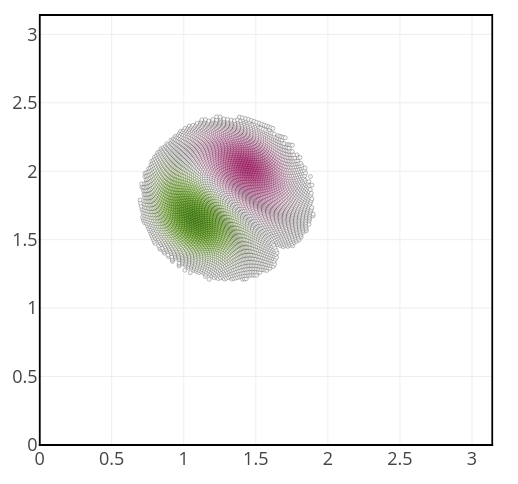
\includegraphics[width=\linewidth]{images/app2d/part_eps_0.01.png}
	\end{subfigure}
	\hfill
	\begin{subfigure}{0.3\textwidth}
		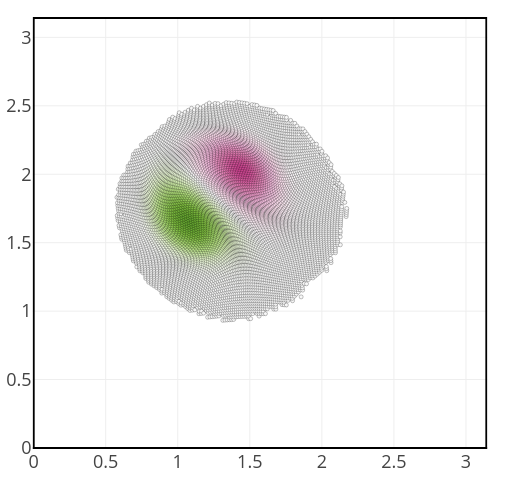
\includegraphics[width=\linewidth]{images/app2d/part_eps_1e-6.png}
	\end{subfigure}
	\caption{Effect of the parameter $\varepsilon_\omega$ on the particle discretization of the solution for one member. From left to right, results for $\varepsilon_\omega = 0.1, 0.01$, and $1.e-6$.}
	\label{fig:eps_effect}
\end{figure}

For the next paragraphs, if the value is not explicitly changed, we use the nominal parameters described in Table \ref{tab:simu_2d} for the simulation.

\subsection{Assimilation parameters and ensemble generation}

An ensemble of 32 members is created by sampling distributions over the dipole parameters. We sample the radius $R$, the prescribed velocity $U$, the orientation $\theta$, and the barycenter $\bm z_{\text{mean}}$. Additionally, the model viscosity $\nu$ is also sampled. All the distributions are summarized in Table \ref{tab:ens_dipole}. The first six members are plotted in Figure \ref{fig:sample_ens}.

\begin{figure}[ht]
	\centering
	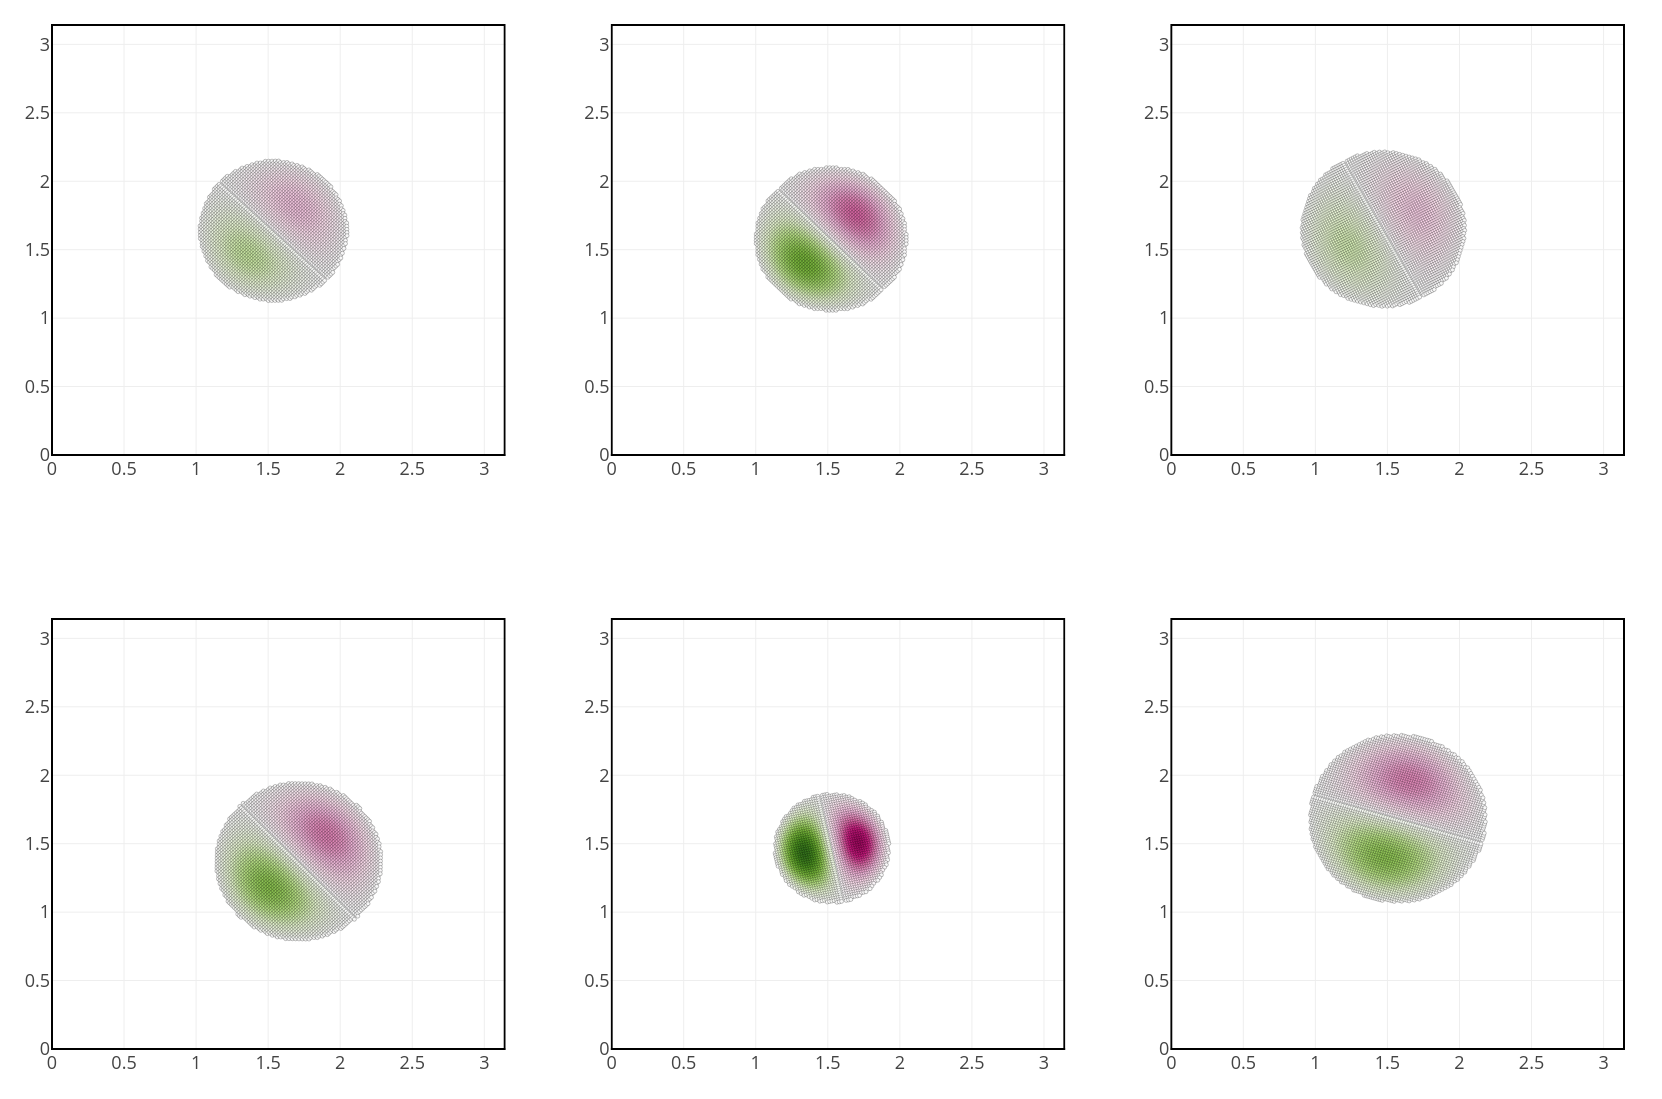
\includegraphics[width=0.7\linewidth]{images/app2d/ensemble_sample.png}
	\caption{Six samples from the initial ensemble.}
	\label{fig:sample_ens}
\end{figure}

The initial vorticity field is first discretized on a regular grid of particles with a characteristic length $d_p$, where each particle receives the circulation $\Gamma_p = \omega(\bm z_p) V_p$, and $V_p = d_p^2$ represents the volume of the particle. The frequency is defined by the assimilation step $dt_a$. The simulation is performed over a duration of $t_f$. All simulation parameters are summarized in Table \ref{tab:simu_2d}.

Observations are collected on a regular grid of size $N_{\text{obs}}$, measuring both components of the velocity. The observations follow a normal distribution $\mathcal N(0, \sigma_{obs}^2 \bm{I}{N{\text{obs}}})$, indicating an ensemble of independent measurements, each characterized by a standard distribution of $\sigma_{obs}$. An example of observed velocity with and without noise is illustrated in Figure \ref{fig:velocity}.

\begin{figure}[htbp]
	\centering
	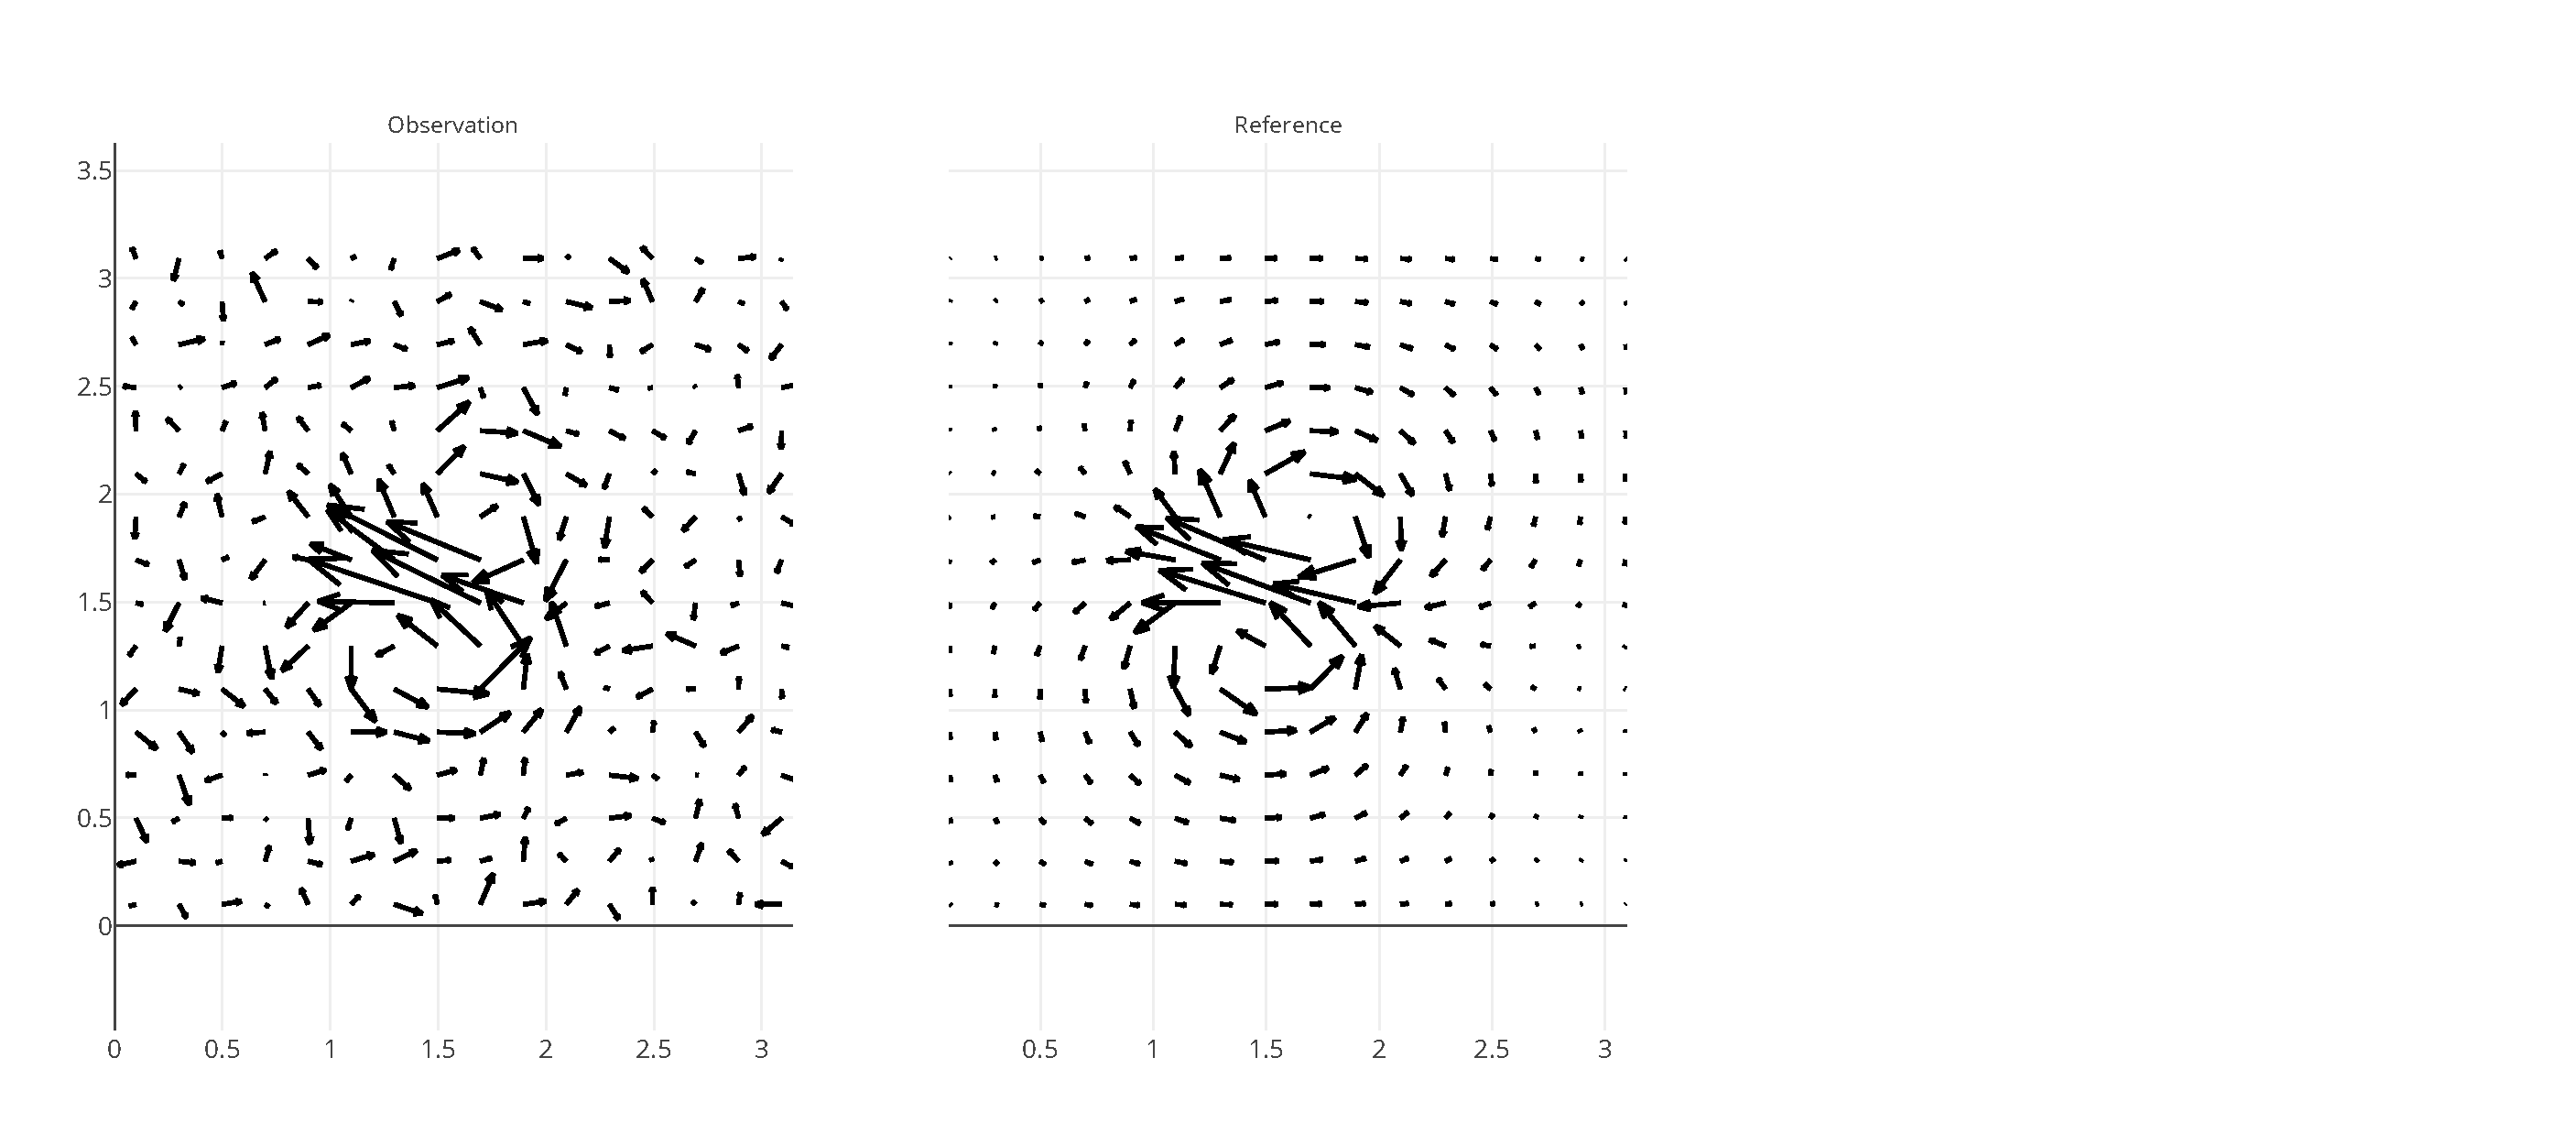
\includegraphics[width=0.8\linewidth]{images/app2d/velocity_ref.pdf}
	\caption{Observed and reference velocity fields. The error on each component is sample from a centred normal distribution with the nominal value $\sigma_{\text{obs}} = 0.05$.}
	\label{fig:velocity}
\end{figure}

We will employ the same metric, the relative \(L_2\)-error, similar to the one-dimensional application in~\ref{eq:L2_error} as well as the absolute \(L_2\)-error. The $L_2$ norm is computed using a quadrature over a regular grid of an ensemble of cells $\mathcal{C}$ such as for any $f \in L_2$

$$
	\norm{f}_{L_2}  = \int_{\Omega} f^2~d\Omega \approx \sum_{c \in \mathcal{C}} f(\z)~V_c
$$~where $\z_c$ is the center of the cell $c$ and $V_c$ the volume of the cell. The grid is still the same for all the simulations.

The Part-EnKF uses here the approximation over the forward particle support. It has been seen to yield relatively good results with efficient time computation. This choice introduces a dependence on the particle discretization. Similar conclusions would be drawn in the following study if a regression operator had been used to approximate the analyzed solution.

\newpage

\subsection{Results}

\begin{figure}[htbp]
	\centering
	\begin{subfigure}{0.49\linewidth}
		\includegraphics*[width=\linewidth]{images/app2d/field_error_w_assim.pdf}
	\end{subfigure}
	\begin{subfigure}{0.49\linewidth}
		\includegraphics*[width=\linewidth]{images/app2d/viscosity_error_w_assim.pdf}
	\end{subfigure}
	\caption{Error curves through assimilation steps. Left: \(L_2\)-error of the field, Right: Error for the viscosity parameter. With Part-EnKF in blue and Remesh-EnKF in red.}
	\label{fig:assim_time}
\end{figure}

We start by analyzing the assimilation error over time. Figure \ref{fig:assim_time} illustrates the relative error throughout the assimilation process for the nominal set of parameters, demonstrating comparable results for both filters, as well as for the assimilation of state and model viscosity. Additionally, Figure \ref{fig:visc_time} depicts the evolution of the ensemble distribution for the viscosity parameters. In both cases, the variance and the bias decrease over time. However, the Remesh-EnKF has higher variances compared to the Part-EnKF, particularly at the middle and end stages of assimilation. Notably, the filters underestimate the viscosity in the initial assimilation steps. It could be primarily due to the dissipation introduced in the first estimate, which is subsequently offset thanks to the parameter. After subsequent assimilation steps, the parameter finally stabilizes. Nevertheless, the reference always falls within the range of the distribution.

\begin{figure}[htbp]
	\centering
	\begin{subfigure}{0.49\linewidth}
		\includegraphics*[width=\linewidth]{images/app2d/visc_ppf.png}
	\end{subfigure}
	\begin{subfigure}{0.49\linewidth}
		\includegraphics*[width=\linewidth]{images/app2d/visc_rmf.png}
	\end{subfigure}
	\caption{Evolution of the viscosity ensemble through assimilation. Left: for the Part-EnKF, Right: for the Remesh-EnKF. In blue the ensemble values, in red the estimate and black the reference.}
	\label{fig:visc_time}
\end{figure}

We assess the performances of the different filters by evaluating the convergence of the error with respect to the assimilation and the simulation parameters. Additionally, we added a filter called Part-Grid-EnKF. This last filter combined the approximation process of the Part-EnKF but on a regularly spaced particle discretization like the Remesh-EnKF filter. This filter will allow us to better show if the difference between the filters is due to the Part-EnKF discretization or the particle approximation.
First, we observe the convergence rate concerning data assimilation parameters: the observation precision, which is \(1/\sigma_{\text{obs}}^2\), the number of observations \(n_{\text{obs}}\), the number of assimilation step \(N_{\text{assim}}\). The results are regrouped in Figure \ref{fig:assim_params}.
In this context, we first observed that the convergence is more substantial and more regular for the Remesh-EnKF. The convergence is the same at low precision, but for high precision, the error decreases slower for the Part-EnKF and Part-Grid-EnKF. In fact, the observed high reduction of variances and the high bias suggest a collapse of the state of the ensemble to a suboptimal solution. Nevertheless, the viscosity errors are all comparable. This observation leads to the conclusion that the approximation step bounds the error of the state.
As concern the convergence for other assimilation parameters \(n_{\text{obs}}\), \(\sigma_{\text{obs}}\), the conclusion is quite similar. The field error decreases with \(n_{\text{obs}}\), \(\sigma_{\text{obs}}\) for the Remesh-EnKF. The result is more mitigated for the Part-EnKF. Again, it confirms that the Part-EnKF fails to converge as successfully as the Remesh-EnKF.
Finally, we note that the converge with respect to \(n_{\text{obs}}\), \(\sigma_{\text{obs}}\) are less regular even for the Remesh-EnKF. This observation is probably mainly due to the fact that the measures and assimilation steps are regularly spaced over space and time. In fact, the number of measures over the dipole at time $t$ is low, and the relative position could have a relatively high impact on the assimilation.

\begin{figure}[htbp]
	\begin{subfigure}{0.45\textwidth}
		\captionsetup{labelformat=empty}
		\centering
		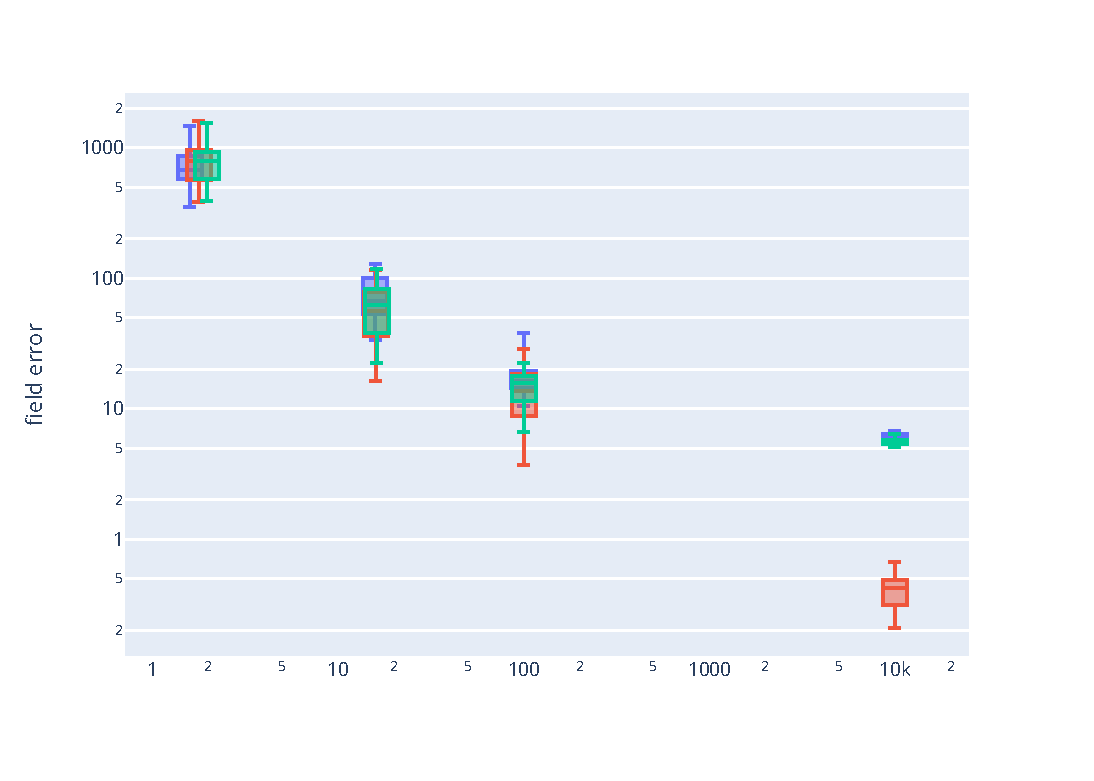
\includegraphics[width=\linewidth]{./images/app2d/MSE_obs_precision_box.pdf}
		\caption{state error w.r.t. $1/\sigma_{\text{obs}}^2$}
	\end{subfigure}
	\hfill
	\begin{subfigure}{0.45\textwidth}
		\captionsetup{labelformat=empty}
		\centering
		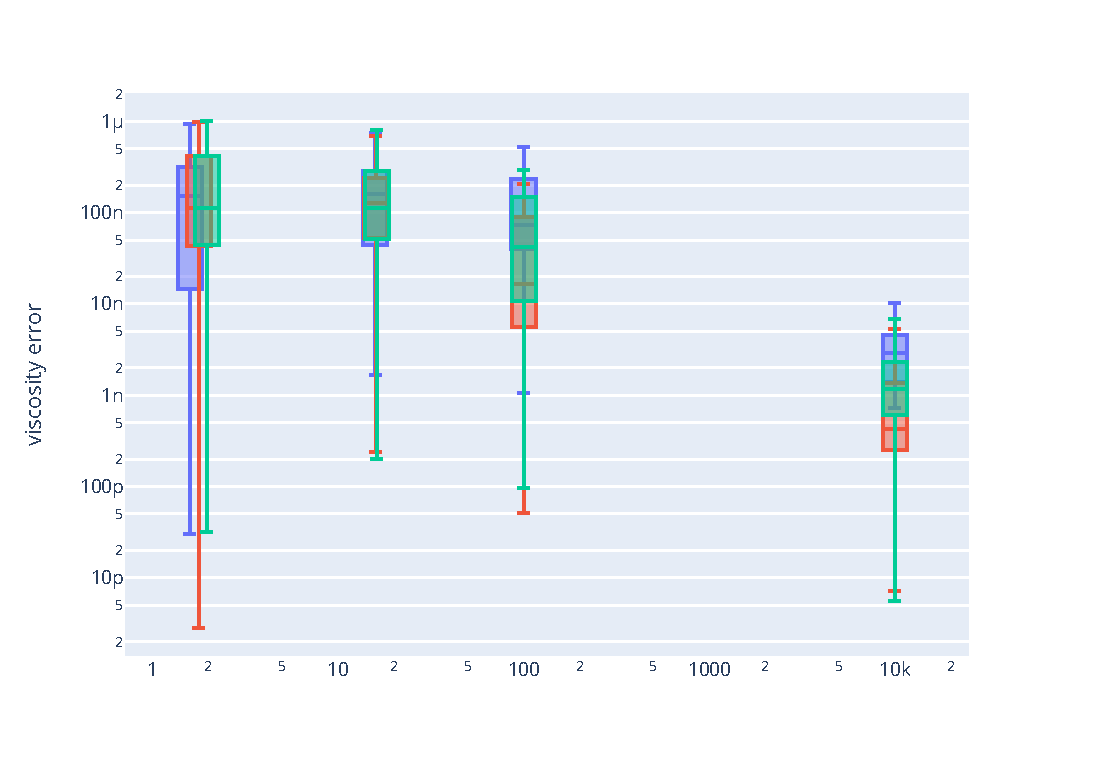
\includegraphics[width=\linewidth]{./images/app2d/MSE_visc_obs_precision_box.pdf}
		\caption{viscosity error w.r.t $1/\sigma_{\text{obs}}^2$}
		\label{fig:obs_precision}
	\end{subfigure}
	\begin{subfigure}{0.45\textwidth}
		\centering
		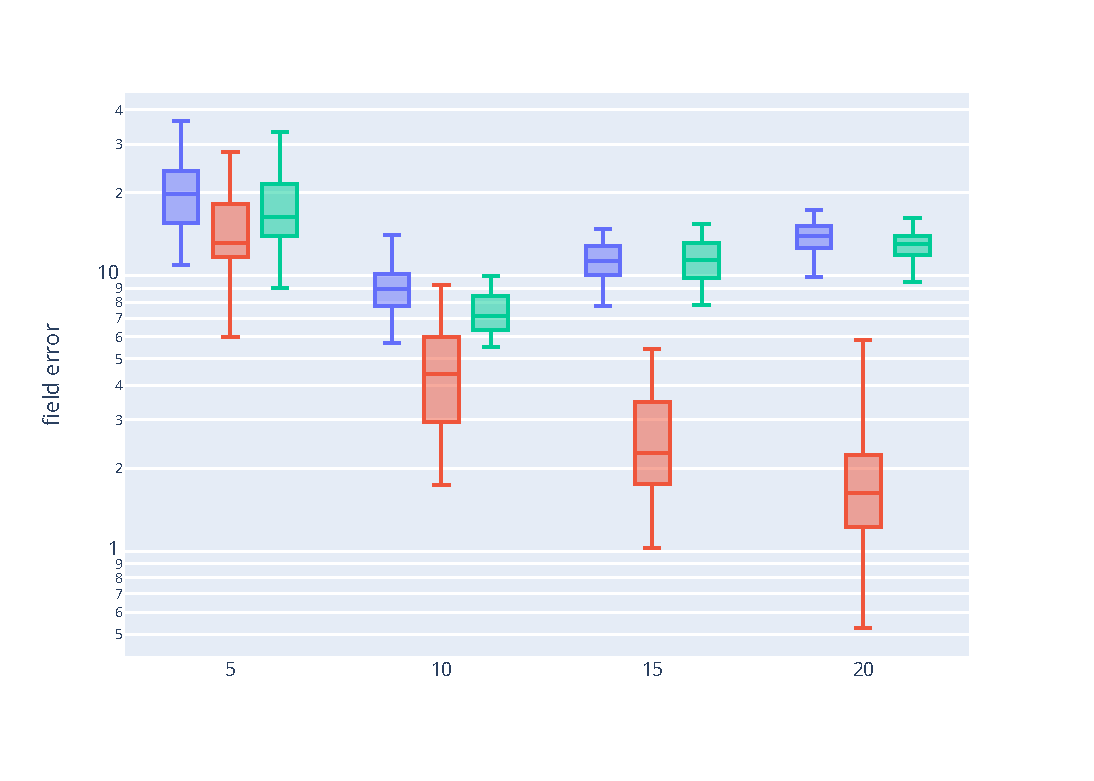
\includegraphics[width=\linewidth]{./images/app2d/MSE_na_box.pdf}
		\captionsetup{labelformat=empty}
		\caption{state error w.r.t. $N_{\text{assim}}$}
	\end{subfigure}
	\hfill
	\begin{subfigure}{0.45\textwidth}
		\centering
		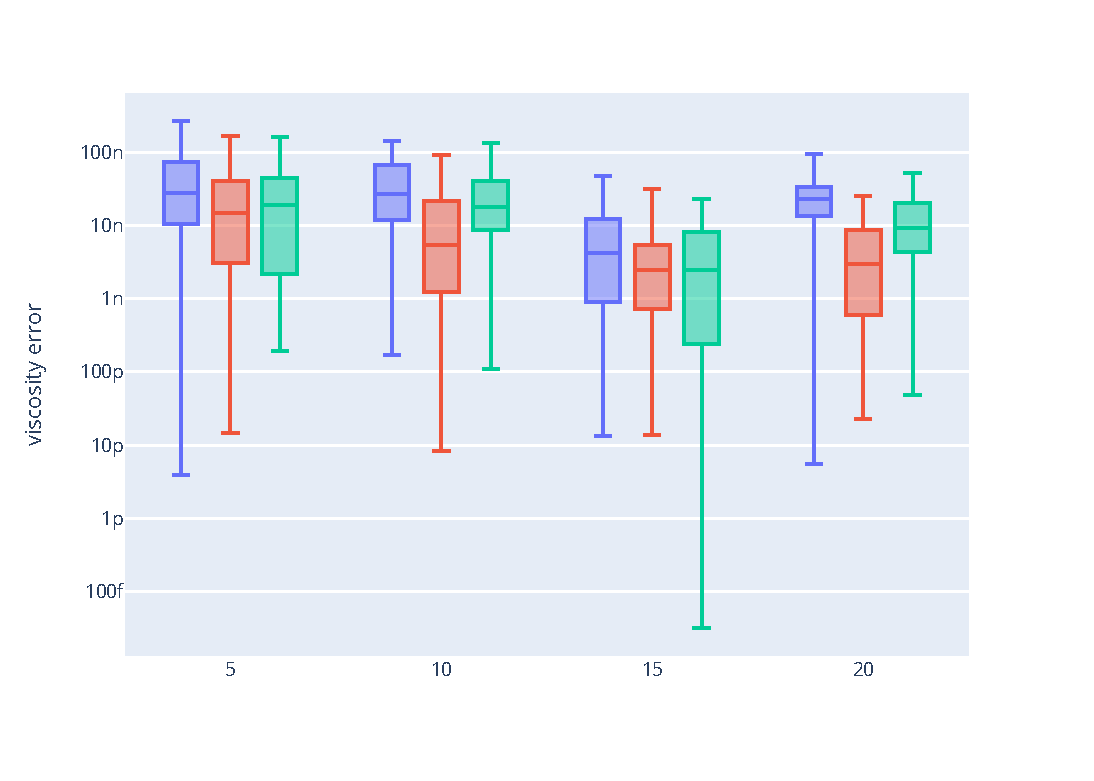
\includegraphics[width=\linewidth]{./images/app2d/MSE_visc_na_box.pdf}
		\captionsetup{labelformat=empty}
		\label{fig:na}
		\caption{viscosity error w.r.t. $N_{\text{assim}}$}
	\end{subfigure}
	\begin{subfigure}{0.48\textwidth}
		\captionsetup{labelformat=empty}
		\centering
		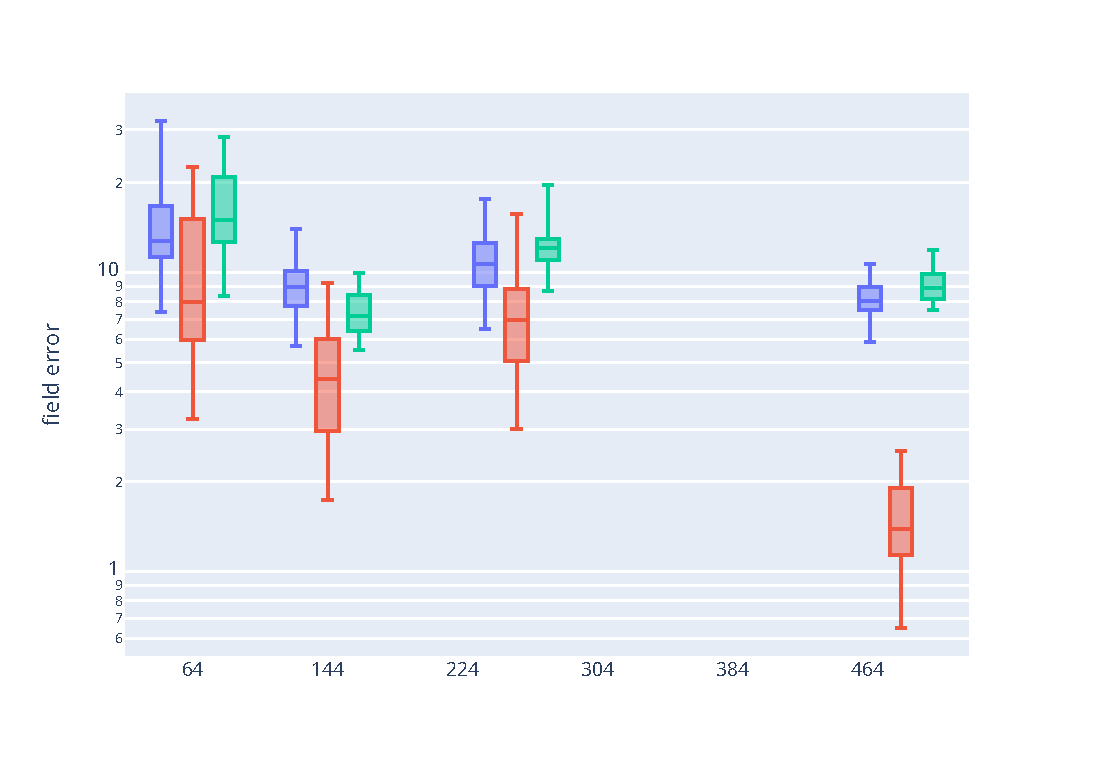
\includegraphics[width=\linewidth]{./images/app2d/MSE_nobs_box.pdf}
		\caption{state error w.r.t. $N_{\text{obs}}$}
	\end{subfigure}
	\hfill
	\begin{subfigure}{0.45\textwidth}
		\captionsetup{labelformat=empty}
		\centering
		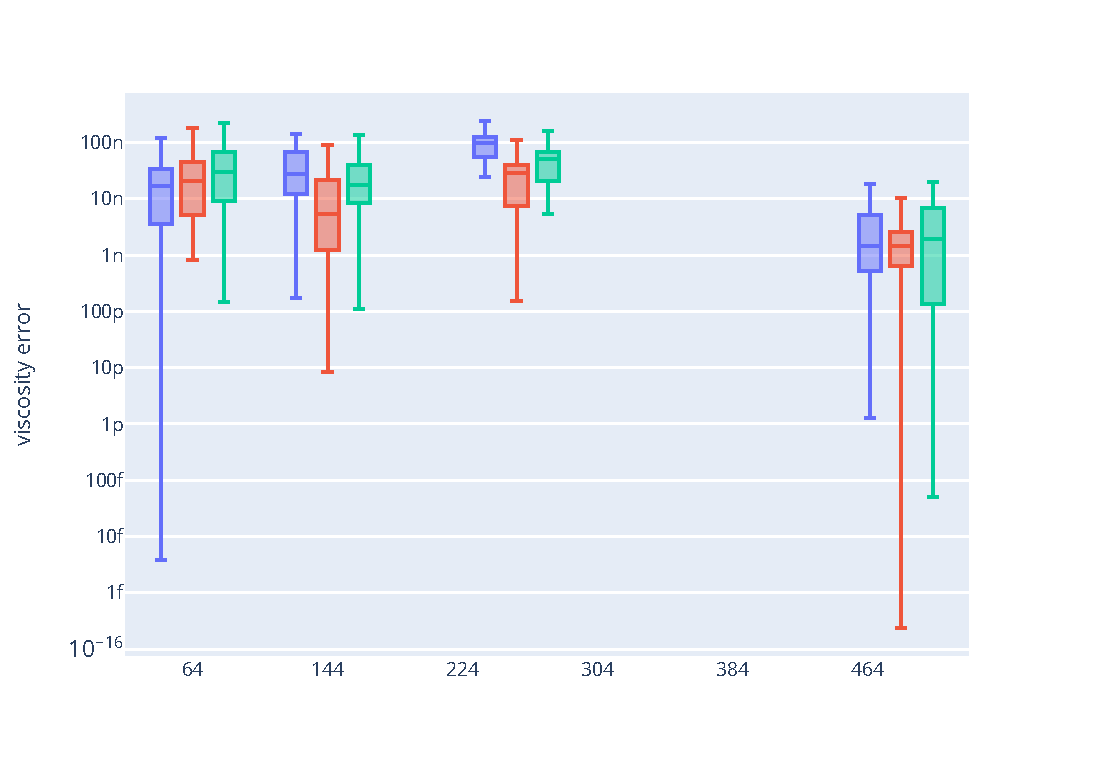
\includegraphics[width=\linewidth]{./images/app2d/MSE_visc_nobs_box.pdf}
		\caption{viscosity error w.r.t $N_{\text{obs}}$}
		\label{fig:nobs}
	\end{subfigure}
	\caption{Error curves for different assimilation parameters. Left: The normalize $L_2$ error for the vorticity field. Right: The normalize error on viscosity.}
	\label{fig:assim_params}
\end{figure}

To better understand the differences, we also evaluate the evolution of the error with respect to particle discretization parameters. For the Part-EnKF, remember that each member has its own particle discretization that flows according to the dipole direction and velocity. Each analyzed member's solutions are then respectively projected on their member discretization. However, this scheme could introduce different sources of error. First, due to particle irregularity in the particle distribution, it introduced severe approximation that led to errors between the analyzed and the approximated solution. Even more seriously, certain parts of the solution may vanish as no particle in the support can interpolate it. This effect could be appreciated on several samples of the ensemble where the analysis is projected on a non-conforming particle discretization. For instance, we analyzed the first assimilation step of one member for the different filters. If the analyzed field is known over the space domain, we observed in Figure~\ref{fig:assim_member} that the Remesh-Filter and Part-Grid-EnKF are only able to interpolate the entire solution. The Part-EnKF is not entirely able to interpolate the solution with the forecast member discretization.
Moreover, some distortions observed in the particle distribution are not in line with the analyzed field flow. These remarks are more critical when the forecast step is longer, leading to high errors, or when the size of the support is lower. Moreover, the approximation of Section \ref{regressionOperator} will introduce the approximation error function of the size of the particles. For instance, the particle will not conserve the total circulation due to a quadrature error, which is the opposite case for the Remesh-EnKF filter.

\begin{figure}[h!]
	\centering
	\begin{subfigure}{0.45\textwidth}
		\centering
		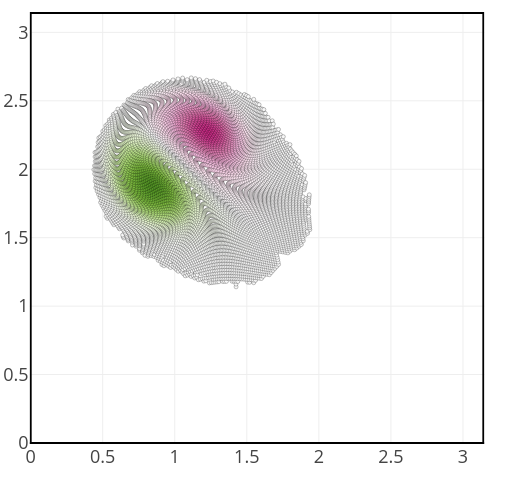
\includegraphics[width=0.8\linewidth]{./images/app2d/assim_member_forecast.png}
	\end{subfigure}
	% \hfill
	\begin{subfigure}{0.45\textwidth}
		\centering
		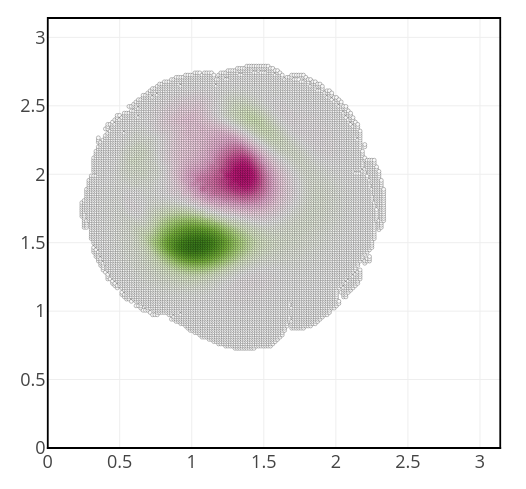
\includegraphics[width=0.8\linewidth]{./images/app2d/assim_member_rmf.png}
	\end{subfigure}
	\begin{subfigure}{0.45\textwidth}
		\centering
		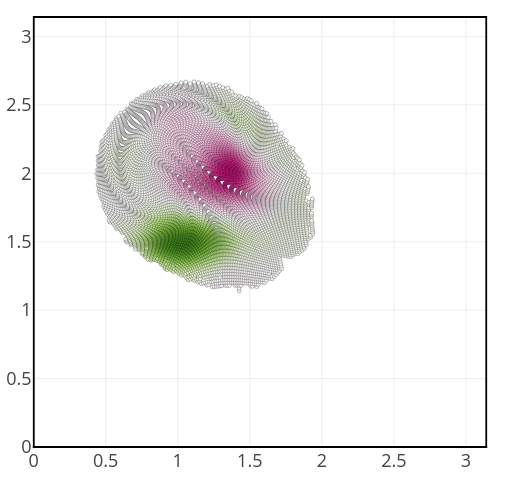
\includegraphics[width=0.8\linewidth]{./images/app2d/assim_member_ppf.png}
	\end{subfigure}
	% \hfill
	\begin{subfigure}{0.45\textwidth}
		\centering
		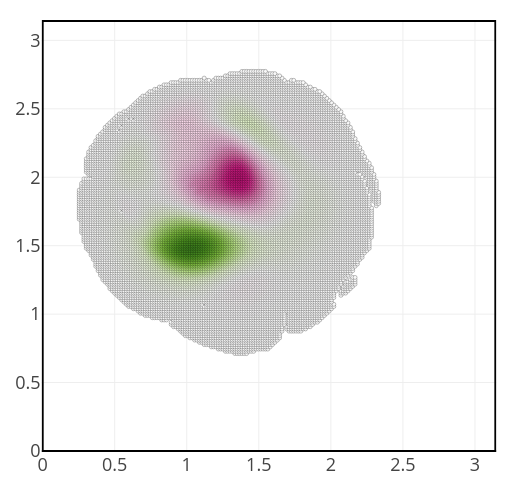
\includegraphics[width=0.8\linewidth]{./images/app2d/assim_member_pgf.png}
	\end{subfigure}
	\caption{Assimilation of one member with a forecast discretization unadapted to the analyses solution. From left to right and up to down: the forecast member, the analyses member with the Remesh-EnKF filter, the analyses member with the Part-EnKF filter and finally the analyses member with the Part-Grid-EnKF. The forecast discretization use by the Part-EnKF is not always a well support of approximation for the analyses and introduce discretization errors.}
	\label{fig:assim_member}
\end{figure}

To evaluate the effect of the size of the support, we varied the value of $\epsilon_{\omega}$. We have seen in Figure~\ref{fig:eps_effect} that this parameter affects the number of particles and, thus, the size of the support. We observe relatively bad results for very high $\epsilon_{\omega}$ because the solution can not be approximated over all the dipole and leads to a significant difference with Remesh-EnKF/Part-Grid-EnKF and variance inside the ensemble. However, the error stabilizes rapidly by decreasing the threshold. A relatively low effect is also observed on the Remesh-EnKF due to truncation errors at the border of the dipole solution.

Thanks to the Part-Grid-EnKF, we could better decompose the error. On the one hand, the difference between the Part-EnKF and the Part-Grid-EnKF is linked to the support and the distortion of the particle distribution. On the other hand, the remaining difference between Part-Grid-EnKF is due to the particle approximation error. This hypothesis is confirmed by analyzing the error with respect to the particle size $d_p$ in Figure \ref{fig:simu_parameters_error}. We observe that the error for Part-EnKF and Part-Grid-EnKF increases proportionally with $d_p$ as for the approximation error. The same order of magnitude for the different filters is observed is observed for relatively small particle sizes. This confirmed the high effect of the particle approximation in this case. Using a regression operator to approximate the analyzed solution should alleviate this effect provided other particle discretization considerations (distortion, support size) as illustrated in Part~\ref{App_1D} and the choice of an adequate penalty coefficient to succeed in approximating the solution.

\begin{figure}[htbp]
	\centering

	\begin{subfigure}{0.48\textwidth}
		\centering
		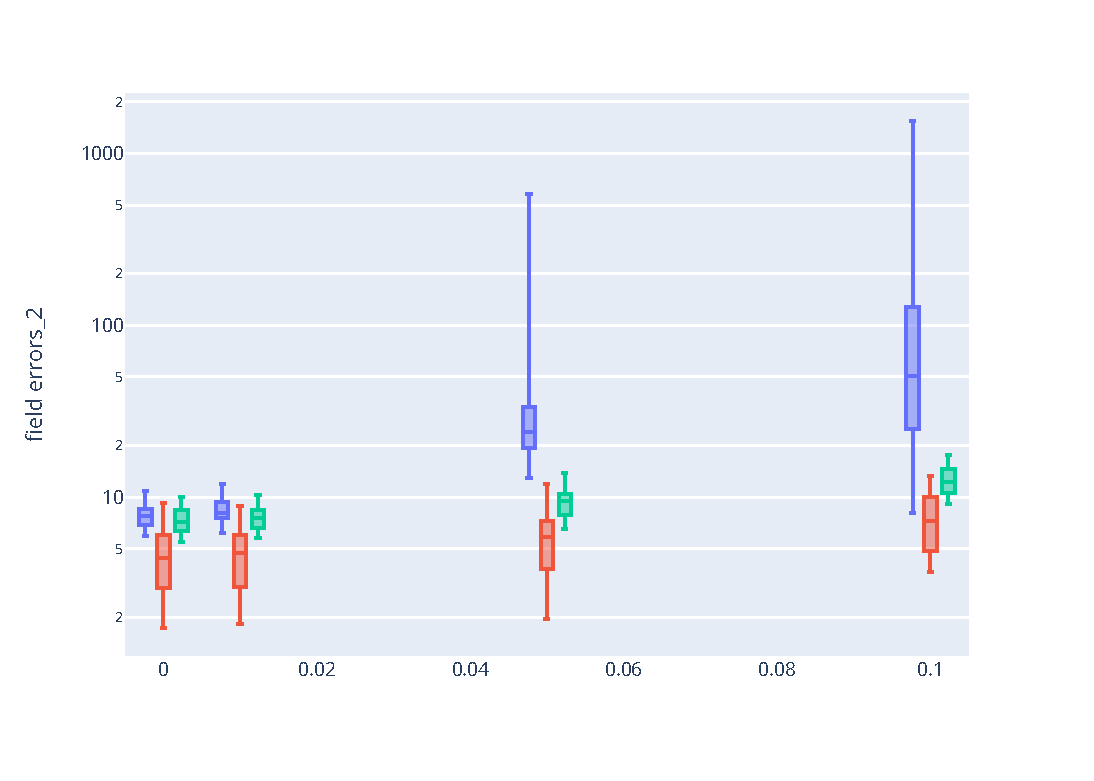
\includegraphics[width=\linewidth]{./images/app2d/MSE_eps_omega_box.pdf}
		\captionsetup{labelformat=empty}
		\caption{state error w.r.t. $\varepsilon_{\omega}$}
		\label{fig:eps_omega}
	\end{subfigure}
	\hfill
	\begin{subfigure}{0.48\textwidth}
		\centering
		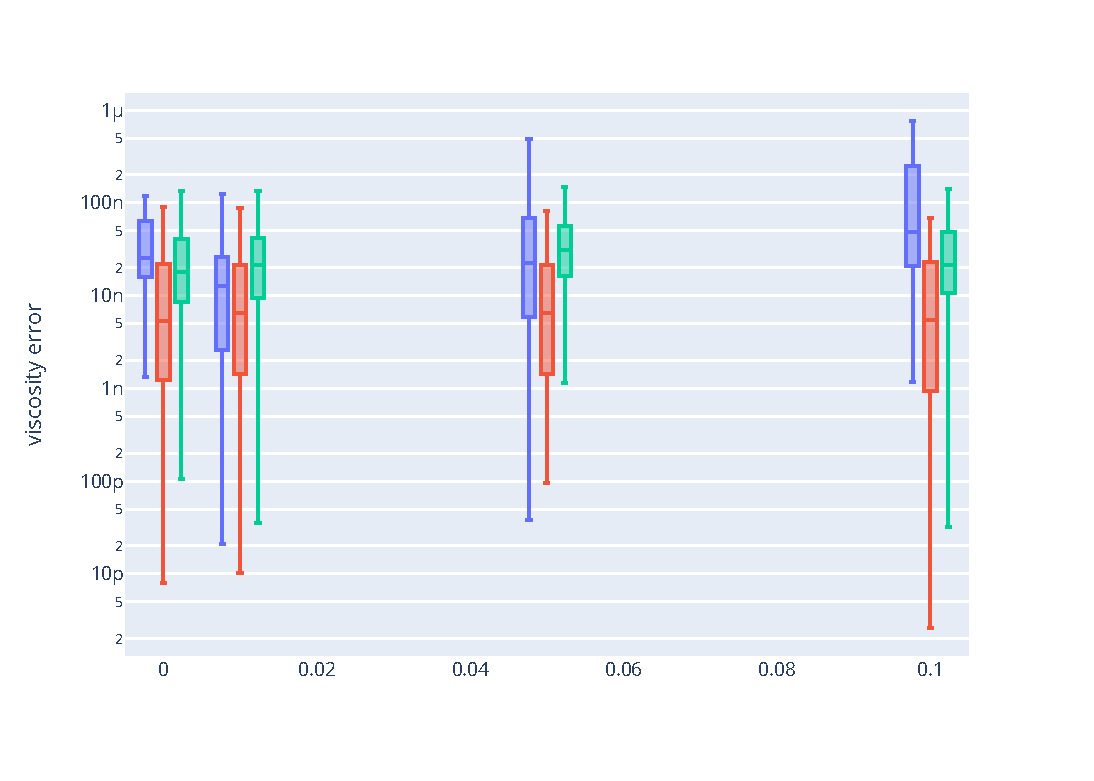
\includegraphics[width=\linewidth]{./images/app2d/MSE_visc_eps_omega_box.pdf}
		\captionsetup{labelformat=empty}
		\caption{viscosity error w.r.t. $\varepsilon_{\omega}$}
		\label{fig:eps_omega_visc}
	\end{subfigure}
	\begin{subfigure}{0.48\textwidth}
		\centering
		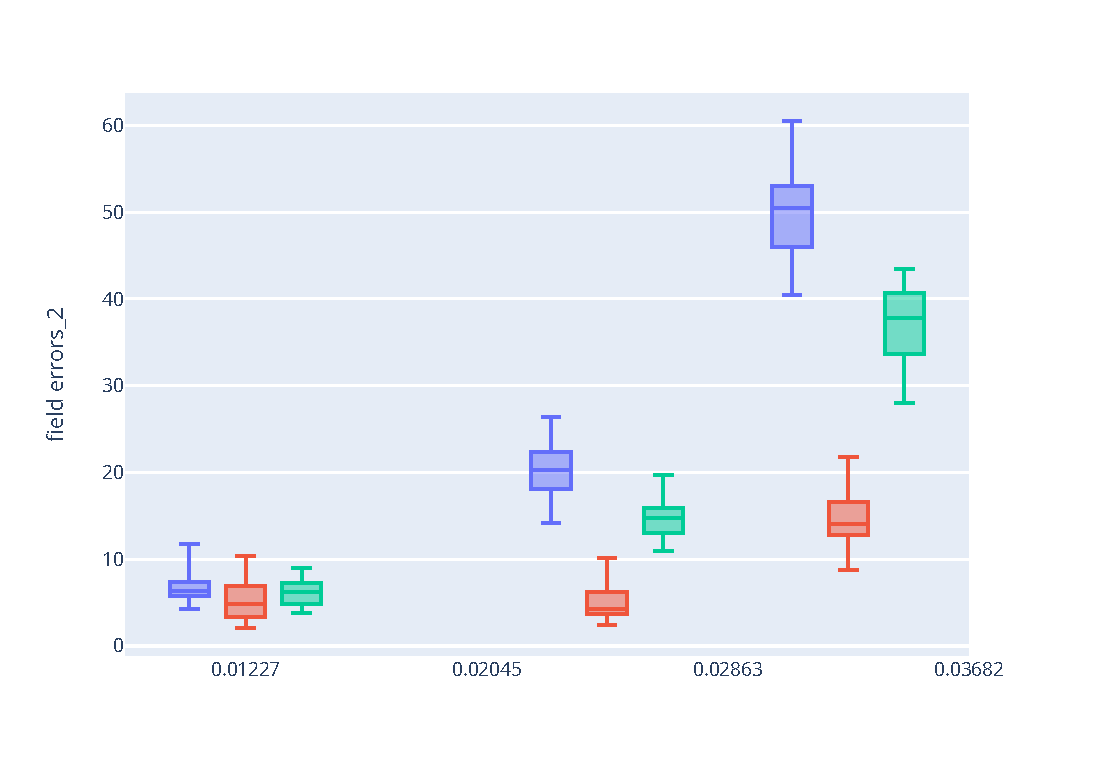
\includegraphics[width=\linewidth]{./images/app2d/MSE_dp_box.pdf}
		\captionsetup{labelformat=empty}
		\caption{state error w.r.t. $d_p$}
		\label{fig:np_visc}
	\end{subfigure}
	\hfill
	\begin{subfigure}{0.48\textwidth}
		\centering
		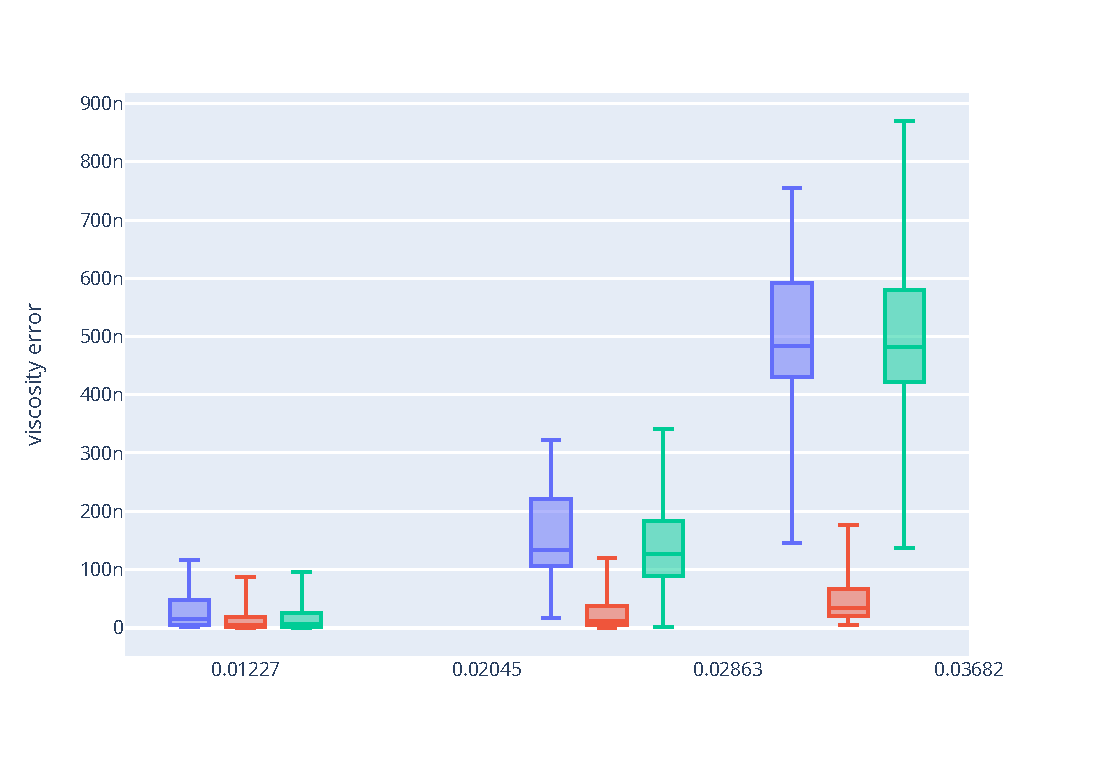
\includegraphics[width=\linewidth]{./images/app2d/MSE_visc_dp_box.pdf}
		\captionsetup{labelformat=empty}
		\caption{viscosity error w.r.t. $d_p$}
		\label{fig:np}
	\end{subfigure}
	\caption{Error curves for simulation parameters. The effect of $\varepsilon_{\omega}$ on the error is particularly observed on high value. The Part-EnKF error is strongly linked to $d_p$ through the particle approximation error.}
	\label{fig:simu_parameters_error}
\end{figure}

This discussion pointed out the high dependency of the Part-EnKF on particle discretization. As it could be understood, the particle discretization of a member could be too far from the solution support of particles. This opens the question of the choice of particle discretization. As suggested in Part~\ref{App_1D}, an error estimation could be introduced to choose between the different filters. On the other hand, other approaches could be to select the member with the maximum likelihood estimate to approximate the solution. This proposition has to be evaluated because it could considerably reduce the variance of the ensemble. Moreover, we note that the particle approximation could rapidly have a high effect, as seen in this Part.
\newpage
%We have seen the importance of the support size for the Part-EnKF filter...
